\begin{frame}{Numerical Method implemented}
The numerical method currently implemented are:
  \begin{itemize}
    \item Variational Multiscale Method (VMS)
    \item Streamline upwind Petrov–Galerkin (SUPG)
  \end{itemize} 

Different solution method are available for all of them 
  \begin{itemize}
    \item Non-linear (NLIN)
    \item Linearized-Coupled (LC-VMS)
    \item Linearized-Segregated (LS-VMS)
  \end{itemize} 
\end{frame}


\begin{frame}{Variational Multiscale Method}
  \begin{itemize}
    \item Evolution of the SUPG
    \item Implict LES
    \item It does not need calibration
    \item Residual-based stabilization
  \end{itemize} 
\end{frame}


\begin{frame}{Galkerkin formulation}
Conservation of mass:
\begin{equation}
    \nabla\cdot \Vec{u} = 0
    \label{equfo:cont}
\end{equation}

Conservation of momentum:
\begin{equation}
    \dfrac{\partial \Vec{u}}{\partial t} + (\Vec{u}\cdot\nabla)\Vec{u} + \nabla p - \nu\Delta\Vec{u} - f = 0
        \label{equfo:mom}
\end{equation}

Variational Formulation
\begin{equation}
\begin{split}
  B^G = &   \int_\Omega \dfrac{\partial \Vec{u}}{\partial t}\cdot \Vec{v}\;d\Omega +
    \int_\Omega(\Vec{u}\cdot\nabla)\Vec{u}\cdot \Vec{v} \;d\Omega+ 
    \int_\Omega \nabla (p)\cdot\Vec{v} \;d\Omega + \\
     & + \int_\Omega\nu\nabla\Vec{u}\cdot\nabla\Vec{v} \;d\Omega  -
        \int_\Omega f\cdot\Vec{v} \;d\Omega + 
    \int_\Omega q(\nabla \cdot \Vec{u})\;d\Omega = 0
    \end{split}
    \label{equ:weak}
\end{equation}

\end{frame}

\begin{frame}{Stabilization equations}
\begin{equation}
B^{SUPG}(t, (\Vec{u},p), (\Vec{v},q))  =     \int_\Omega(\tau_m(\Vec{u}\cdot\nabla \Vec{v} +\nabla q)\cdot\Vec{R_m} \;d\Omega+ \int_\Omega \tau_c (\nabla \cdot \Vec{v})R_c \;d\Omega
\label{equ:bsupg}
\end{equation}

\begin{equation}
B^{VMS1}(t, (\Vec{u},p), (\Vec{v},q))  = \int_\Omega (\Vec{u}\cdot\nabla \Vec{v}')\odot(\tau_m \Vec{R_m}) \;d\Omega
\label{equ:bvms1}
\end{equation}


\begin{equation}
B^{VMS2}(t, (\Vec{u},p), (\Vec{v},q))  = -\int_\Omega (\nabla\Vec{v}\odot(\tau_m \Vec{R_m} \otimes \tau_m \Vec{R_m}) \;d\Omega
\label{equ:bvms2}
\end{equation}

\end{frame}


\begin{frame}{Stabilization parameters}

\begin{equation}
\tau_m =\bigg( \dfrac{4}{\Delta t^2} + \Vec{u}\cdot{G}\Vec{u} + C_I \nu^2 {G}:{G} \bigg)^{-1/2}
\label{equ:taum}
\end{equation}

\begin{equation}
\tau_c = (\tau_c\Vec{g}\cdot\Vec{g})^{-1}
\label{equ:tauc}
\end{equation}

Where G is the inverse of the gradient of the map cell.
For a cubed shaped element, with $h$ the edge length, $G_{ij} =\dfrac{1}{h^2}\delta_{ij}$, where $\delta_{ij}$ is the Kronecker delta.

\end{frame}


\begin{frame}{Linearization}
Using Taylor's expansion for velocity:
\begin{equation}
    \Vec{u}_{adv} = 2.1875 u^{n} - 2.1875 u^{n-1} + 1.3125 u^{n-2} - 0.3125 u^{n-3} 
    \label{equlin:taylor_exp}
\end{equation}

\begin{equation}
 (\Vec{u}\cdot\nabla)\Vec{u} \Rightarrow  (\Vec{u}_{adv}\cdot\nabla)\Vec{u} 
\end{equation}

$\Vec{u}_{adv}$ used also for computing stabilization parameters


\end{frame}

\begin{frame}{Linearization}
\begin{equation}
  \begin{split}
  B^G(t, (\Vec{u},p), (\Vec{v},q))  = &  \int_\Omega \dfrac{\partial \Vec{u}}{\partial t}\cdot \Vec{v}\;d\Omega +
      \int_\Omega(\Vec{u}_{adv}\cdot\nabla)\Vec{u}\cdot \Vec{v} \;d\Omega+ 
      \int_\Omega \nabla (p)\cdot\Vec{v} \;d\Omega + \\
      & + \int_\Omega\nu\nabla\Vec{u}\cdot\nabla\Vec{v} \;d\Omega  -
          \int_\Omega f\cdot\Vec{v} \;d\Omega + 
      \int_\Omega q(\nabla \cdot \Vec{u})\;d\Omega
  \end{split}
      \label{equ:Bglin}
  \end{equation}
  
  \begin{equation}
  B^{SUPG,lin}(t, (\Vec{u},p), (\Vec{v},q))  =     \int_\Omega(\tau_m(\Vec{u}_{adv}\cdot\nabla \Vec{v} +\nabla q)\cdot\Vec{R_{m,lin}} \;d\Omega+ \int_\Omega \tau_c (\nabla \cdot \Vec{v})R_c \;d\Omega
  \label{equ:bsupglin}
  \end{equation}
  
  \begin{equation}
  B^{VMS1,lin}(t, (\Vec{u},p), (\Vec{v},q))  = \int_\Omega (\Vec{u}_{adv}\cdot\nabla \Vec{v}')\odot(\tau_m \Vec{R_{m,lin}}) \;d\Omega
  \label{equ:bvms1lin}
  \end{equation}
\end{frame}


\begin{frame}{ODE Solver}
Employing $\theta$-method for time marching. $\theta=0.5$ for velocity and $\theta=1.0$ for pressure to avoid un-smoothed oscillations
\begin{figure}
  \centering
  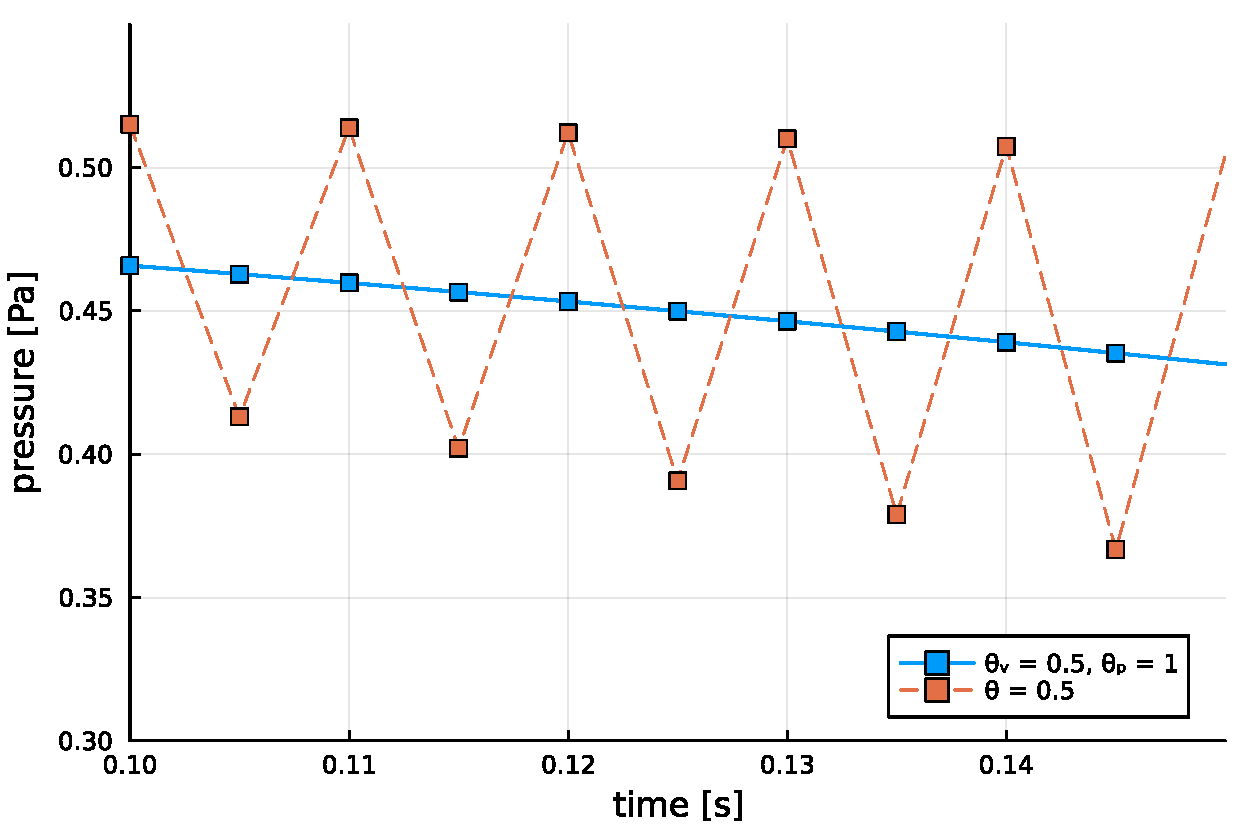
\includegraphics[width=0.45\textwidth]{Theta_stab_nstab.pdf}
  \caption{Pressure oscillations}
\end{figure} 
\end{frame}


\begin{frame}{Segregated formulation}
\begin{equation}
  T\dfrac{\partial \Vec{x}}{\partial t} + A \Vec{x} = 0
  \label{equseg:eq1}
\end{equation}
Applying the $\theta$-method

\begin{equation}
      T\dfrac{\partial \Vec{x}}{\partial t} = - A \Vec{x}
      \label{equseg:eq2}
\end{equation}


\begin{equation}
      T\dfrac{\Vec{x}^{n+1}-\Vec{x}^{n}}{\Delta t} = - \bigg ( A \Vec{x}^{n+1}\theta + A\Vec{x}^n(1-\theta) \bigg )
      \label{equseg:eq3}
\end{equation}

\begin{equation}
      \bigg (\dfrac{T}{\Delta t}+A\theta \bigg )(\Vec{x}^{n+1}-\Vec{x}^{n}) = - A \Vec{x}^{n}
\end{equation}
  
\end{frame}

\begin{frame}{Matrices splitting}

  Splitting the problem in solving velocity and pressure field:
\begin{equation}
  A = \begin{bmatrix}
A_{pp} & A_{pu}\\
A_{up} & A_{uu}
\end{bmatrix}
\end{equation}

\begin{equation}
  T = \begin{bmatrix}
  0 & T_{pu}\\
  0 & T_{uu}
\end{bmatrix}
\end{equation}


Thanks to the stabilization the matrix $A_{pp}$ is nonzero. This translates into nonzero diagonal elements, reducing the conditioning number of the matrix and improving the overall stability of the method.

\end{frame}


\begin{frame}
Introducing the time step increments and the acceleration terms:
$$\Delta u = u^{n+1}-u^{n}$$
$$\Delta p = p^{n+1}-p^{n}$$
$$a = \Delta u / \Delta t$$

The linear system will be solved in an iterative manner. Two following iterations are marked as $m$ and $m+1$, and the difference between two following iteration is:
$$\Delta a = a^{m+1}-a^m$$
$$\Delta p^{m+1} = a^{m+1}-a^m$$
$$u^m=u^n+\Delta t a^m$$
$$p^m = p^n + \sum_{i=0}^m \Delta p^i$$
\end{frame}

\begin{frame}
  \begin{equation}
    \begin{split}
    (T_{uu}+\theta \Delta t A_{uu})\bm{\Delta a^*} = -A_{uu}u^m- Au_{up}p^m - (T_{uu}+\theta\Delta t A_{uu})a^m+A_{uu}\Delta t a^m +\\+ A_{uu}\Delta t a^m + (1-\theta)A_{up}\sum_{i=0}^m \Delta p^i  
  \end{split}
  \label{equseg:mom1}
\end{equation}

\begin{equation}
  \begin{split}
  \bigg( (T_{pu}+\Delta t A_{pu})(T_{uu}+\theta\Delta t A_{uu})^{-1} \theta A_{up} - App \bigg ) \bm{\Delta p^{m+1}} = \\= T_{pu}\Delta a^* + A_{pu}(u^m+\Delta t\Delta a^*)+A_{pp}p^m+T_{pu}a^m
\end{split}
\label{equseg:cont1}
\end{equation}
\end{frame}

\begin{frame}
  It is possible to apply a multicorrector-predictor iterative scheme. At the beginning of each time step the velocity, pressure, and acceleration are initialized as:
\begin{itemize}
\item $u^0 = u^n$
\item $p^0 = p^n$
\item $a^0 = 0$
\item $\sum_{i=0}^m \Delta p^i = 0$
\end{itemize}

Then the iterative process begins:

\begin{enumerate}
    \item Solve linear system \eqref{equseg:mom1} for $\Delta a^*$
    \item Solve linear system \eqref{equseg:cont1} for $\Delta p^{m+1}$
    \item Compute $\Delta a = \Delta a^* - (T_{uu}+\theta\Delta t A_{uu})^{-1}\theta A_{up}  \Delta p^{m+1}$
    \item Update $a^{m+1} = a^m + \Delta a$
    \item Update $u^{m+1} = u^m + \Delta a \Delta t$
    \item Update $p^{m+1} = p^m +\Delta p^{m+1}$
\end{enumerate}

\end{frame}